\section{Dataset}

\subsection{CelebA} \label{sec:CelebA}

CelebA is a large-scale face attributes dataset with more than 200K celebrity images, each with 40 attribute annotations. The images in this dataset cover large pose variations and background clutter. CelebA has large diversities, large quantities, and rich annotations, including \textbf{5,000 celebrity identities}, \textbf{202,599 face images}, and \textbf{40 binary attributes} annotations per image. The dataset can be employed as the training and test sets for the following computer vision tasks: face attribute recognition, face detection, landmark (or facial part) localization, and face editing/synthesis.

% insert the image of the dataset
\begin{figure}[h]
\centering
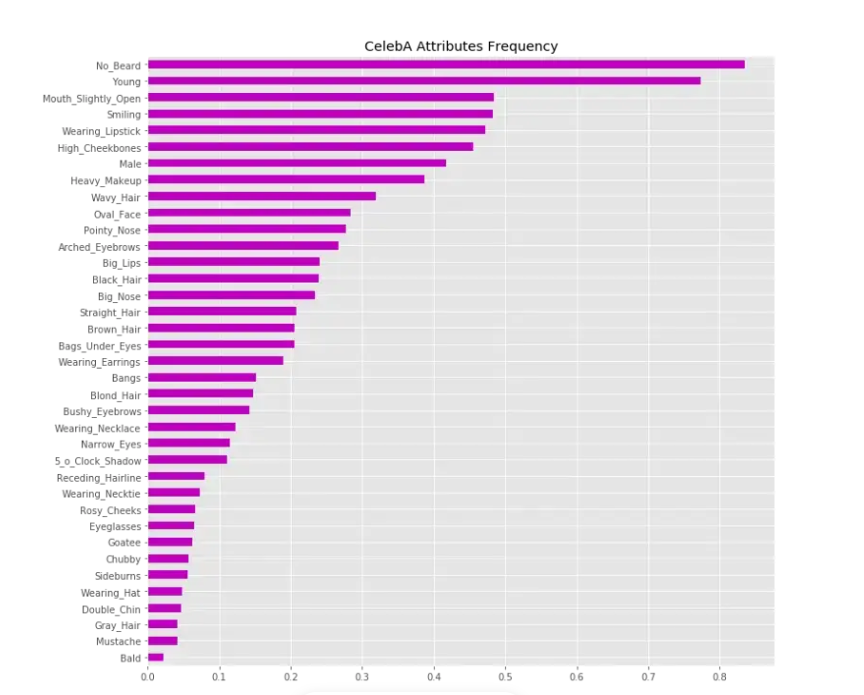
\includegraphics[width=0.5\textwidth]{CelebA_stat.png}
\caption{CelebA dataset distribution}
\label{fig:CelebA_stat}
\end{figure}

\begin{figure}[htbp]
    \centering
    \begin{subfigure}{0.4\textwidth}
        \centering
        \includegraphics[width=1\textwidth]{CelebA.png}
        \caption{CelebA dataset cover large pose variations}
    \end{subfigure}
    \qquad
    \begin{subfigure}{0.4\textwidth}
        \centering
        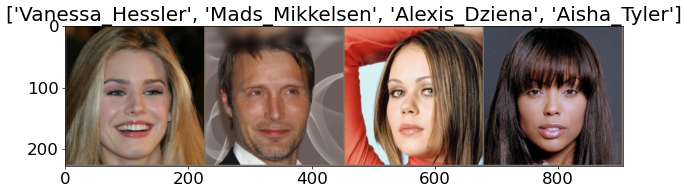
\includegraphics[width=1\textwidth]{CelebA_usage.png}
        \caption{CelebA in face recognition}
    \end{subfigure}
    \caption{An excerpt from CelebA dataset}
    \label{fig:CelebA}
\end{figure}

In this project, we utilized a subset of CelebA as the face recognition model's dataset. The dataset includes 5696 images of 307 different people, with 4429 images used for training and 1267 images used for testing.

\subsection{Private Dataset}

For a better presentation, we also constructed a private dataset consisting 121 images of all team members. The photos were cropped from 3 videos, which were uniformly sampled to 40 frames each to vary the facial expression. In each frame, the face image is detected by package Mediapipe and then stored in the local device. \footnote{This process is done in Data\_generation.ipynb.ipynb.}

The private dataset and CelebA dataset togetherly form the training and testing dataset of our face recognition model.
